% \documentclass[supercite]{upcthesis}
\documentclass[12pt]{ctexart}
% \documentclass[10pt]{article}
\usepackage{lipsum}
\usepackage{listings}
\usepackage{xcolor}
\usepackage{makecell}
\usepackage{amsmath}
\usepackage{mathtools}
\usepackage{amsfonts,amssymb}
\usepackage{subfigure}
\usepackage{enumerate}
\usepackage{graphicx}
\usepackage{float}%使用此命令来固定图片的位置
\usepackage{epstopdf}
\usepackage{etoolbox}
\usepackage{titlesec}

\usepackage[titles,subfigure]{tocloft}
\thispagestyle{empty}
\usepackage{geometry}
\geometry{left=3.18cm,right=3.18cm,top=2.54cm,bottom=2.54cm}
\pagestyle{plain}	
\usepackage{setspace}
\date{}
\usepackage{fancyhdr}
\usepackage{titlesec}
\usepackage {xcolor}

\usepackage{xeCJK}
% \setCJKmainfont[BoldFont=STZhongsong, ItalicFont=STKaiti]{STSong}
\setmainfont{Times New Roman}
% \setsansfont{Myriad Pro}
\setCJKsansfont[BoldFont=STHeiti]{STXihei}
\setCJKmonofont{STFangsong}

\usepackage{array}%需要该宏包
\renewcommand\arraystretch{2}
\newfontfamily\sectionef{Arial}	% 设置Arial字体		
% \newCJKfontfamily\sectioncf{STXihei}	% 设置黑体
\titleformat{\section}{\center\zihao{-3}\heiti\sectionef}{第\,\thesection\,节}{1em}{}% 设置一级标题居中,中文字体为黑体,英文字体为Arial,字号为小三号
\titleformat*{\subsection}{\zihao{4}\heiti\sectionef}	% 设置二级标题中文字体为黑体,英文字体为Arial字号为四号
 
\usepackage[bookmarks=true,colorlinks,linkcolor=black,
citecolor=black]{hyperref}			% 设置超链接
 
\usepackage[superscript]{cite}		% 引入参考文献格式包
\bibliographystyle{mybst}		% 参考文献格式采用自制的mybst
\newcommand{\upcite}[1]{\textsuperscript{\textsuperscript{
			\citeleft}\cite{#1}\textsuperscript{\citeright}}}	% 设置参考文献序号格式
 
\usepackage{setspace}
\usepackage{geometry}		
\geometry{left=3.2cm,right=3.2cm,top=4.0cm,bottom=4.0cm}	% 设置页边距
\usepackage{fancyhdr}		% 设置页眉
\pagestyle{fancy}	
\fancyhf{}													
\cfoot{\thepage}				% 设置页码
\CTEXsetup[name = {第,节}]{section}		% 设置章节格式
\renewcommand{\sectionmark}[1]{\markboth{第\thesection 节\quad % 设置页眉内容为章标题
		\ #1}{}}
 
%---------------------------cover.tex-------------------------------
\thispagestyle{empty}						%  当前页不显示页码
%------------------------abstract_cn.tex-------------------------------
\setcounter{page}{1}						% 设置当前页页码编号从1开始计数
\pagenumbering{Roman}						% 设置页码字体为大写罗马字体
%----------------------------main.tex-------------------------------
\setcounter{page}{1}						% 设置当前页页码编号从1开始计数
\pagenumbering{arabic}						% 设置页码字体为小写阿拉伯字体
 
 
 
\begin{document}
	%\maketitle
	\include{cover}								% 封面
	\fancyhead[C]{\leftmark}					% 设置页眉内容为章标题
	\include{contents}							% 目录
	
	\setcounter{page}{1}
	\pagenumbering{arabic}
	
	\markboth{leftmark}{rightmark}
	\include{conclusion_reference_thanks}
	
	

	
		\begin{center}
		\quad \\
		\vskip 3.5cm
		\heiti \fontsize{30}{20} 付费问答系统设计文档%毕\quad 业\quad 论\quad 文
		\vskip 1.5cm
		 \zihao{4} 程爽 \quad 董一凡 \quad 韩佳俊\quad 王洋
	\end{center}
	\vskip 3.5cm
	\vskip 1.5cm
\tableofcontents
\newpage
\section{需求分析}
\subsection{项目背景}
随着互联网技术的发展,人们能便利地从互联网获取大量信息,而信息爆炸和信息无序也增加了人们检索、筛选、辨别信息的成本。移动支付的普及也促成了知识服务从免费过渡到付费——从免费资源获取到“一问一答”的点对点精准问答。本项目旨在提供一个付费问答系统。在该系统中,提问者可以向指定回答者发起提问并支付,问题经过审核系统审核后,将会被推送给回答者, 回答者在限定的时间内进行作答。问答服务完成后将会自动对订单进行结算,回答者和平台会进行 收入和佣金分配。
\subsection{实现特性}
通过仔细阅读和整理原始需求文档,我们以蓝图的形式将需求实现的功能列举如下(功能基本和API接口相对应),每个功能可以进行相对独立的开发以及测试。总体上,我们设计了3个蓝图:用户蓝图、订单蓝图和审核系统蓝图。3个蓝图相互独立,分别管理各自的数据库设计、API接口设计和API管理设计。具体详情如下:
\subsubsection{用户管理}
\begin{enumerate}[a)]
	\item 普通用户管理\begin{itemize}
		\item 支持用户的登录与注册
		\item 支持用户进行钱包充值
		\item 支持用户修改密码
		\item 支持用户通过邮箱找回密码
		\item 支持用户修改邮箱和修改用户头像
		\item 支持用户查看自己的用户名头像余额等信息
	\end{itemize}
	\item 回答者管理\begin{itemize}
		\item 支持普通用户升级为回答者
		\item 支持所有回答者信息展示
		\item 支持按照回答者用户名寻找回答者
		\item 支持回答修改自己的领域以及定价等信息
		\item 支持回答者查看自己的领域以及定价等信息
		\item 支持回答者按月维度查看收入统计
		\item 支持用户收入统计更新
		\item 支持用户和回答者之间的即时通信
	\end{itemize}
\end{enumerate}
\subsubsection{订单管理}
\begin{itemize}
	\item 支持提问者向指定回答者发起提问,创建订单并支付订单
	\item 支持向审核系统返回所有订单
	\item 支持审核系统审核员对订单进行审核
	\item 支持审核不成功时触发系统退款
	\item 支持回答者查看已经审核通过且属于自己的订单
	\item 支持回答者在限定时间内接单
	\item 支持回答者拒绝接单
	\item 支持回答者不在指定时间内接单时触发系统退款
	\item 支持回答者接单后在限定时间内作答
	\item 支持提问者和回答者结束订单
	\item 支持回答时间超出限定后自动结束订单
	\item 支持订单完成指定时长后订单进行结算
	\item 支持审核人删除已经审核完成的订单
	\item 支持回答者删除已经完成的订单
	\item 支持提问者删除已经完成的订单
	\item 支持用户按照自己是提问者还是回答者身份筛选查看订单
	\item 支持用户按照订单状态筛选查看订单
\end{itemize}
\subsubsection{审核系统}
\begin{enumerate}[a)]
	\item  Admin管理员\begin{itemize}
		\item 支持系统处理化admin管理员,账号与密码均为”root”
		\item 支持admin管理员修改密码
		\item 支持admin管理员添加新的管理员并由系统生成初始密码
		\item 支持admin管理员修改/更新管理员角色的权限
		\item 支持admin删除指定的其他管理员
		\item 支持admin管理修改系统配置参数\begin{itemize}
			\item 答者定价区间
			\item 回答者接单时长
			\item 回答者等待时间时长
			\item 最多回答次数
			\item 最长回答时间
		\end{itemize}
	\end{itemize}
	\item 审核员\begin{itemize}
		\item 支持管理员查看信息
		\item 支持管理员修改密码
		\item 支持管理员查看系统参数
	\end{itemize}
\end{enumerate}
\subsubsection{非功能需求}
\begin{itemize}
	\item 后端API接口文档
	\item 基于issue的细粒度开发
	\item Merge request时的代码审核机制
\end{itemize}
\subsection{用例}
采用图的形式描述一些主要功能。
\subsubsection{用户管理}
具体功能可以参见1.2.1里面的实现特性。主要包含对用户的注册、升级以及用户信息等方面的管理,用例图如下:
\begin{figure}[H]
	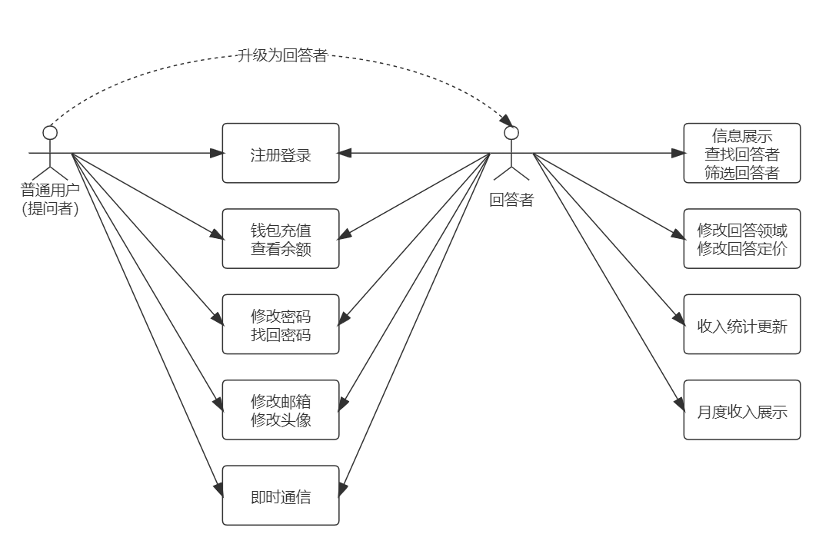
\includegraphics{1.png}\caption{用户管理用例图}
\end{figure}
\subsubsection{订单管理}
具体功能可以参见1.2.2里面的实现特性。主要包含订单创建、订单审核、订单接收、订单结算等相关的功能,用例图如下:
\begin{figure}[H]
	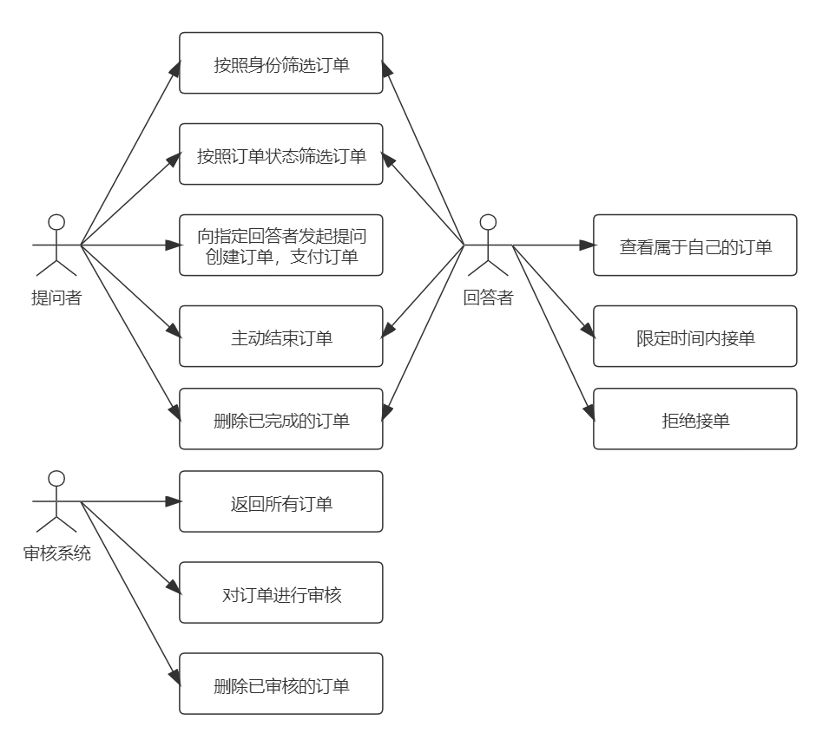
\includegraphics{3.png}\caption{订单管理用例图}
\end{figure}
\subsubsection{审核系统}
具体功能可以参见1.2.3里面的实现特性。主要包含管理员的注册、更新以及对系统参数等方面的管理,用例图如下:
\begin{figure}[H]
	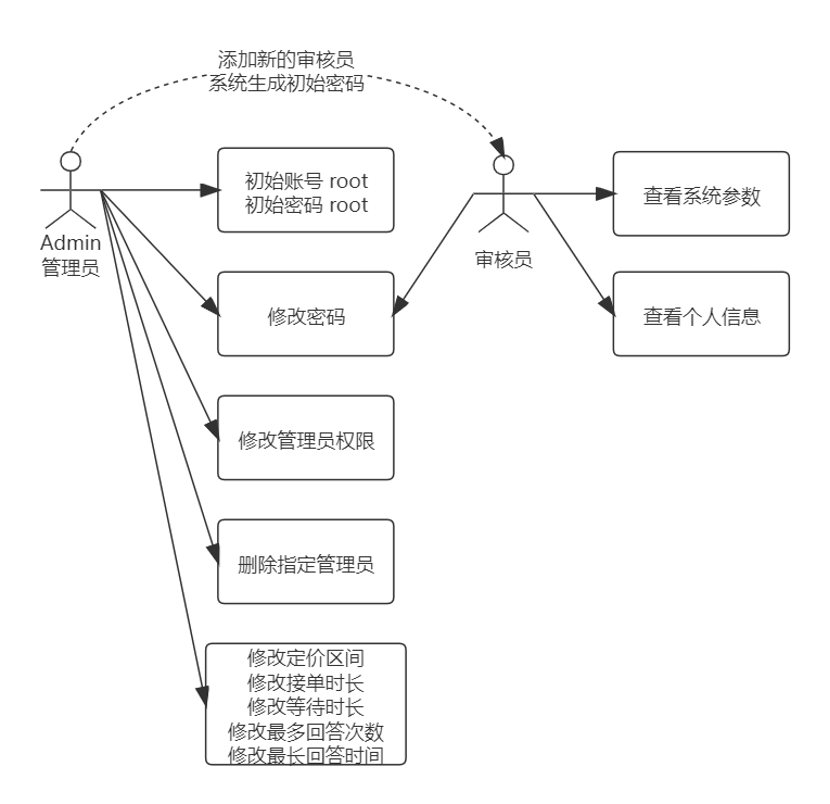
\includegraphics{4.png}\caption{审核系统用例图}
\end{figure}
\subsection{交互流程}
整个流程严格按照项目需求文档的描述:
\begin{figure}[H]
	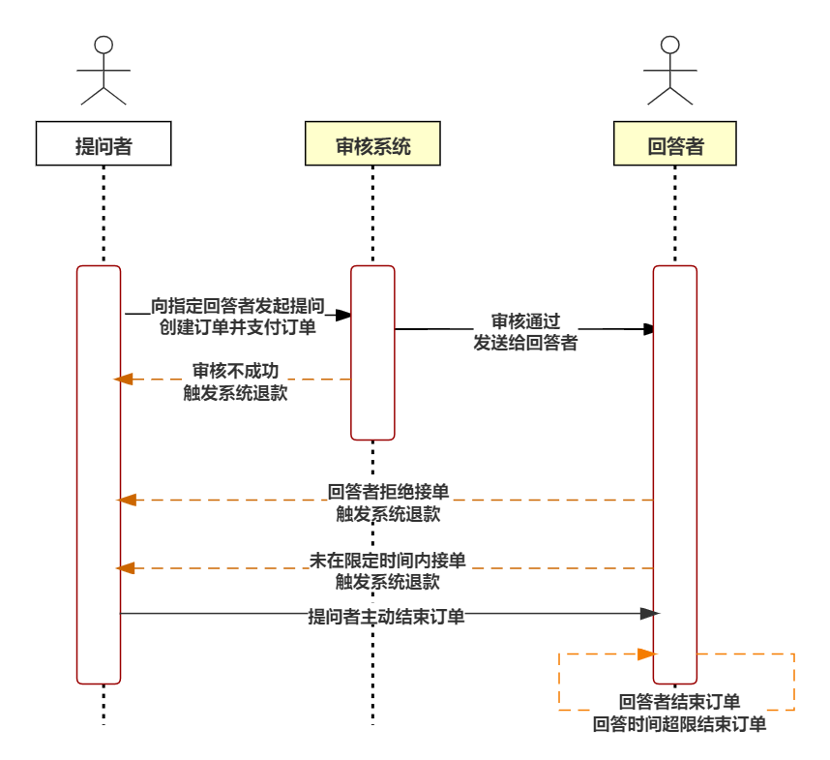
\includegraphics{2.png}\caption{主要交互流程}
\end{figure}

\section{模块及接口设计}
项目介绍分为前端和后端两部分,前端源码位于根目录/vue目录下,后端源码位于根目录/api目录下。前端使用Element-UI开发,主要用于处理用户的交互;后端使用Flask开发,主要分为功能接口、工具函数和单元测试三个部分。其中功能接口可分为用户模块、订单模块、管理员模块。
\subsection{用户模块}
用户模块的代码位于/api/authentication文件中,该模块实现了和用户直接相关的功能。
\subsubsection{注册}
本系统的大部分功能只对处于登录状态的用户开放。为了登录本系统,使用者需要先注册用户账号。与用户注册相关的接口设计如下:
\begin{itemize}
	\item Register:支持任意非用户发起注册请求。发起注册请求后会立刻产生新用户,默认身份为提问者,并在数据库中保存。为了根据用户名区分不同的用户,用户名会进行查重,已经注册过的用户名无法被其他用户注册使用。另外注册时填写的邮箱也不可以重复注册,绑定过的邮箱无法被其他用户绑定,以便实现找回密码服务。
\end{itemize}
\subsubsection{登录}
拥有账号的使用者可以通过用户名和密码登录本系统。与用户登录相关的接口设计如下:
\begin{itemize}
	\item Login:支持用户使用正确的用户名和密码登录。用户名或密码输入错误的用户不能成功登录。
\end{itemize}
\subsubsection{修改信息}
已注册用户可以通过忘记密码功能,利用绑定的邮箱找回密码。与用户找回密码相关的接口设计如下:
\begin{itemize}
	\item Find Password:支持用户使用正确的用户名和绑定过的邮箱找回密码,输入邮箱后会在短时间内将验证码发送到指定邮箱,填写正确的验证码并输入新密码后可以完成找回密码功能。
\end{itemize}
已登录的用户可以修改密码、修改邮箱、升级成为回答者等。与用户修改信息相关的接口设计如下:
\begin{itemize}
	\item Modify Password:支持修改用户登录密码,输入正确的用户名和原密码,再设置新密码。
	\item Modify Email:支持修改用户绑定邮箱,输入新邮箱。
	\item Modify Photo:支持修改用户头像,上传不大于64kb的图片。
	\item Update:支持用户从提问者升级为回答者,输入回答领域和个人简介以及回答定价。
	\item Modify Answerer:支持用户修改回答者信息,包括修改回答领域、修改个人简介、修改回答定价。
\end{itemize}
\subsubsection{用户聊天}
本系统的一个重要功能就是用户间的聊天功能,提问者和回答者通过聊天系统解答订单问题。该部分依托于腾讯云IM,使用的相关接口如下:
\begin{itemize}
	\item User Login:支持用户登录腾讯云,在登录系统时会同时登录腾讯云。
	\item Send Message:支持用户发送聊天信息,默认发送的消息为未读状态。
	\item Accept Message:支持用户接受聊天信息,默认显示的消息为未读状态。
	\item User List:支持用户进入聊天系统时可以和系统内所有用户进行聊天,聊天系统的UI设计类似微信网页版。
	\item Unread Message:支持将未读消息转为已读状态,触发条件为点击聊天用户列表其他用户头像。
\end{itemize}
\subsection{订单模块}
订单模块的代码位于/api/order文件中,该模块实现了与订单直接相关的功能。
\subsubsection{添加订单}
提问者可以向喜欢的回答者提问,输入提问标题以及提问内容之后就会在数据库中添加新的订单,接口设计如下:
\begin{itemize}
	\item Add Order:支持提问者通过输入提问标题以及提问内容生成新订单,并存储在数据库相应表中。
\end{itemize}
\subsubsection{订单操作}
提问者可以取消提问,可以手动完成订单;回答者可以拒绝接单,可以接受订单,可以手动完成订单(订单需要先被管理员审核才会显示在前端,这部分在第三部分阐述),接口设计如下:
\begin{itemize}
	\item Complete Order:支持提问者或回答者手动完成订单,并将数据库中对应的订单状态改为已完成。
	\item Change Order:支持提问者或回答者操作订单,包括接单、拒单、取消提问等,并将数据库中对应的订单状态改为对应的状态。
	\item First Answer:支持回答者接单后首次回答问题,并将数据库中对应的订单相应表项记录为已完成首次回答。
\end{itemize}
\subsubsection{订单结算}
在用户手动结算订单或订单回答时间超过设定时间后,会进入订单结算阶段,相关的接口设计如下:
\begin{itemize}
	\item Order Settlement:支持在订单完成三天后将对应金额款数打到回答者的账户中。(由于演示需要在实际工程中设置为了1分钟)
\end{itemize}
\subsection{管理员模块}
管理远模块的代码位于/api/admin文件中,在问答系统之外还有一个审核系统,审核系统主要处理订单审核以及系统全局变量的设定。
\subsubsection{admin}
admin管理员负责修改全局变量,相关的接口设计如下:
\begin{itemize}
	\item Admin Login:支持admin登录审核系统。
	\item Modify Admin:支持修改admin密码,初始密码为admin,在首次登陆后可以修改密码。
	\item Modify Variable:支持admin修改包括接单时间、首次回答时间、最低定价、最高定价等在内的问答系统全局变量。
\end{itemize}
\subsubsection{审核员操作}
admin管理员负责添加管理员、更新管理员、升级管理员,相关的接口设计如下:
\begin{itemize}
	\item Add Manager:支持admin添加管理员,新添加的管理员默认为未分配科目的审核人员,并自动生成登录密码。
	\item Modify Manager:支持admin改变已分配科目的审核员的科目。
	\item Update Manager:支持admin将已有的未分配科目的管理员升级为审核员,同时设置审核科目类型。
\end{itemize}
\subsubsection{订单审核}
Admin和已分配科目的审核员负责审核订单,相关的接口设计如下:
\begin{itemize}
	\item Check Order:支持审核员审核订单,共有通过和不通过两种状态。
	\item Send Order:支持向审核系统前端发送所有相关科目的未审核的订单,方便审核员进行审核处理。
\end{itemize}
\section{数据库设计}
本项目数据库使用mysql存储数据,数据库中建立多个表用于存储不同类型的信息。共建立以下几种数据表:
\begin{itemize}
	\item 用户表(User): 用于存储用户的个人信息,包括用户名、密码、邮箱、头像等
	\item 回答者表(Answerer):用于存储回答者的个人信息。包括用户名、领域、定价、收入等
	\item 订单表(Orders):用于存储订单的相关信息记录。包括订单id,提问者、回答者、标记、领域等
	\item 管理员表(Admin):用于存储审核系统中管理员的信息。包括用户名、密码等
	\item 系统参数表(System\_configuration):用于存储系统参数。包括最低定价、最高定价、接单等待时间等
\end{itemize}
\subsection{用户表}
用户表用于存储所有用户的账户信息,详情如下:
\begin{table}[H]
	\centering
	\begin{tabular}[]{|p{3cm}<\centering|p{3cm}<\centering|p{3cm}<\centering|p{3cm}<\centering|}
		\hline
		属性 & 类型 & 默认值 & 描述\\
		\hline
		username &	string  &  N/A	& 用户名\\
		\hline
		password\_hash &	string  &	N/A &	密码哈希值\\
		\hline
		email &	string &	N/A &	邮箱\\
		\hline
		photo &	binary	& N/A	& 头像\\
		\hline
		balance &	float &	0	& 余额\\
		\hline
		verification\_code	& string &	N/A &	邮箱验证码\\
		\hline
		confirmed\_at &	datetime &	now &	创建时间\\
		\hline
	\end{tabular}
	\caption{用户表}
\end{table}
\subsection{回答者表}
回答者表用于存储所有回答者的信息,包含回答者领域、定价,个人简介等基础信息,详情如下:
\begin{table}[H]
	\centering
	\begin{tabular}[]{|p{3cm}<\centering|p{3cm}<\centering|p{3cm}<\centering|p{3cm}<\centering|}
		\hline
		属性 & 类型 & 默认值 & 描述\\
		\hline
		username &	string  &  N/A	& 用户名\\
		\hline
		photo &	binary	& N/A	& 头像\\
		\hline
		resume &	string	& N/A	& 个人简介\\
		\hline
		field &	integer &	N/A	 & 领域\\
		\hline
		price &	float &	N/A	& 定价\\
		\hline
		month\_income &	string &	0 &	月收入\\
		\hline
		year\_income	& string &	0	& 年收入\\
		\hline
		confirmed\_at &	datetime &	now &	创建时间\\
		\hline
	\end{tabular}
	\caption{回答者表}
\end{table}
\subsection{订单表}
订单表用于存储所有订单的信息记录,包括订单id、提问者、回答者、订单状态标记等,详情如下:
\begin{table}[H]
	\centering
	\begin{tabular}[]{|p{3cm}<\centering|p{3cm}<\centering|p{3cm}<\centering|p{3cm}<\centering|}
		\hline
		属性 & 类型 & 默认值 & 描述
		\\ \hline
		order\_id &	integer &	N/A &	订单id
		\\ \hline
		title &	string &	N/A &	订单标题
		\\ \hline
		content	& string	& N/A	& 问题内容
		\\ \hline
		questioner &	string &	N/A &	提问者\\ \hline
		answerer &	string &	N/A	& 回答者\\ \hline
		pice &	float &	N/A &	订单价格\\ \hline
		field &	integer &	N/A &	领域\\ \hline
		end\_mark	& integer	& 0 &	状态标记\\ \hline
		first\_answer &	integer &	0	& 是否首次回答\\ \hline
		check\_mark	& integer	& N/A	& 是否通过审核\\ \hline
		confirmed\_at &	datetime &	now &	创建时间\\ \hline
		receive\_at	& datetime	& now	 & 回答者接单时间\\ \hline
	\end{tabular}
	\caption{订单表}
\end{table}
\subsection{管理员表}
管理员表用于存储管理员账户信息,详情如下:
\begin{table}[H]
	\centering
	\begin{tabular}[]{|p{3cm}<\centering|p{3cm}<\centering|p{3cm}<\centering|p{3cm}<\centering|}
		\hline
		属性 & 类型 & 默认值 & 描述
		\\ \hline
		username &	string &	N/A &	用户名\\ \hline
		password\_hash &	string	& N/A	& 密码哈希值\\ \hline
		permission &	integer &	N/A &	是否有管理权限\\ \hline
		management	& integer	& 0	 & 参数是否配置\\ \hline
		confirmed\_at &	datetime &	now &	创建时间\\ \hline
	\end{tabular}
	\caption{管理员表}
\end{table}
\subsection{系统参数表}
管理员表用于存储管理员账户信息,详情如下:
\begin{table}[H]
	\centering
	\begin{tabular}[]{|p{3cm}<\centering|p{3cm}<\centering|p{3cm}<\centering|p{3cm}<\centering|}
		\hline
		属性 & 类型 & 默认值 & 描述
		\\ \hline
		lowest\_prices	& float &	N/A &	最低价 \\ \hline
		top\_prices	& float	& N/A	& 最高价 \\ \hline
		wait\_receive &	float &	N/A &	最长等待接单时间\\ \hline
		wait\_answer	& integer	 & N/A	& 最长首次回答时间\\ \hline
		times\_AQ	& integer &	N/A	 & 最多问答次数\\ \hline
	\end{tabular}
	\caption{管理员表}
\end{table}
\end{document}

